\documentclass[tikz,border=12pt]{standalone}
\usepackage{amsmath}
\usetikzlibrary{arrows.meta,patterns}
\definecolor{meshblue}{RGB}{35,105,170}
\definecolor{body}{RGB}{246,204,151}
\definecolor{flow}{RGB}{185,55,45}
\newcommand{\bodypath}{(0,-1.4)--(3.6,-1.4)--(5,-.55)--(7,-.55)--(7,.55)--(5,.55)--(3.6,1.4)--(0,1.4)--cycle}
\newcommand{\die}{
\fill[pattern=north east lines,pattern color=gray!65] (3.6,1.4)--(5,.55)--(7,.55)--(7,2)--(3.6,2)--cycle;
\fill[pattern=north east lines,pattern color=gray!65] (3.6,-1.4)--(5,-.55)--(7,-.55)--(7,-2)--(3.6,-2)--cycle;
\draw[black!70,thick] (3.6,1.4)--(5,.55)--(7,.55);
\draw[black!70,thick] (3.6,-1.4)--(5,-.55)--(7,-.55);
}

% Web figure typography: 220 dpi gives about 18 px for 6 pt text
% at natural PNG size. Keep text smaller than diagram geometry.
\newcommand{\figtext}{\fontsize{6}{7.5}\selectfont}
\newcommand{\fignote}{\fontsize{5.5}{7}\selectfont}
\newcommand{\figmath}{\fontsize{7}{8.5}\selectfont}
\newcommand{\figtitle}{\fontsize{7.5}{9}\selectfont}
\begin{document}
\hyphenpenalty=10000
\exhyphenpenalty=10000
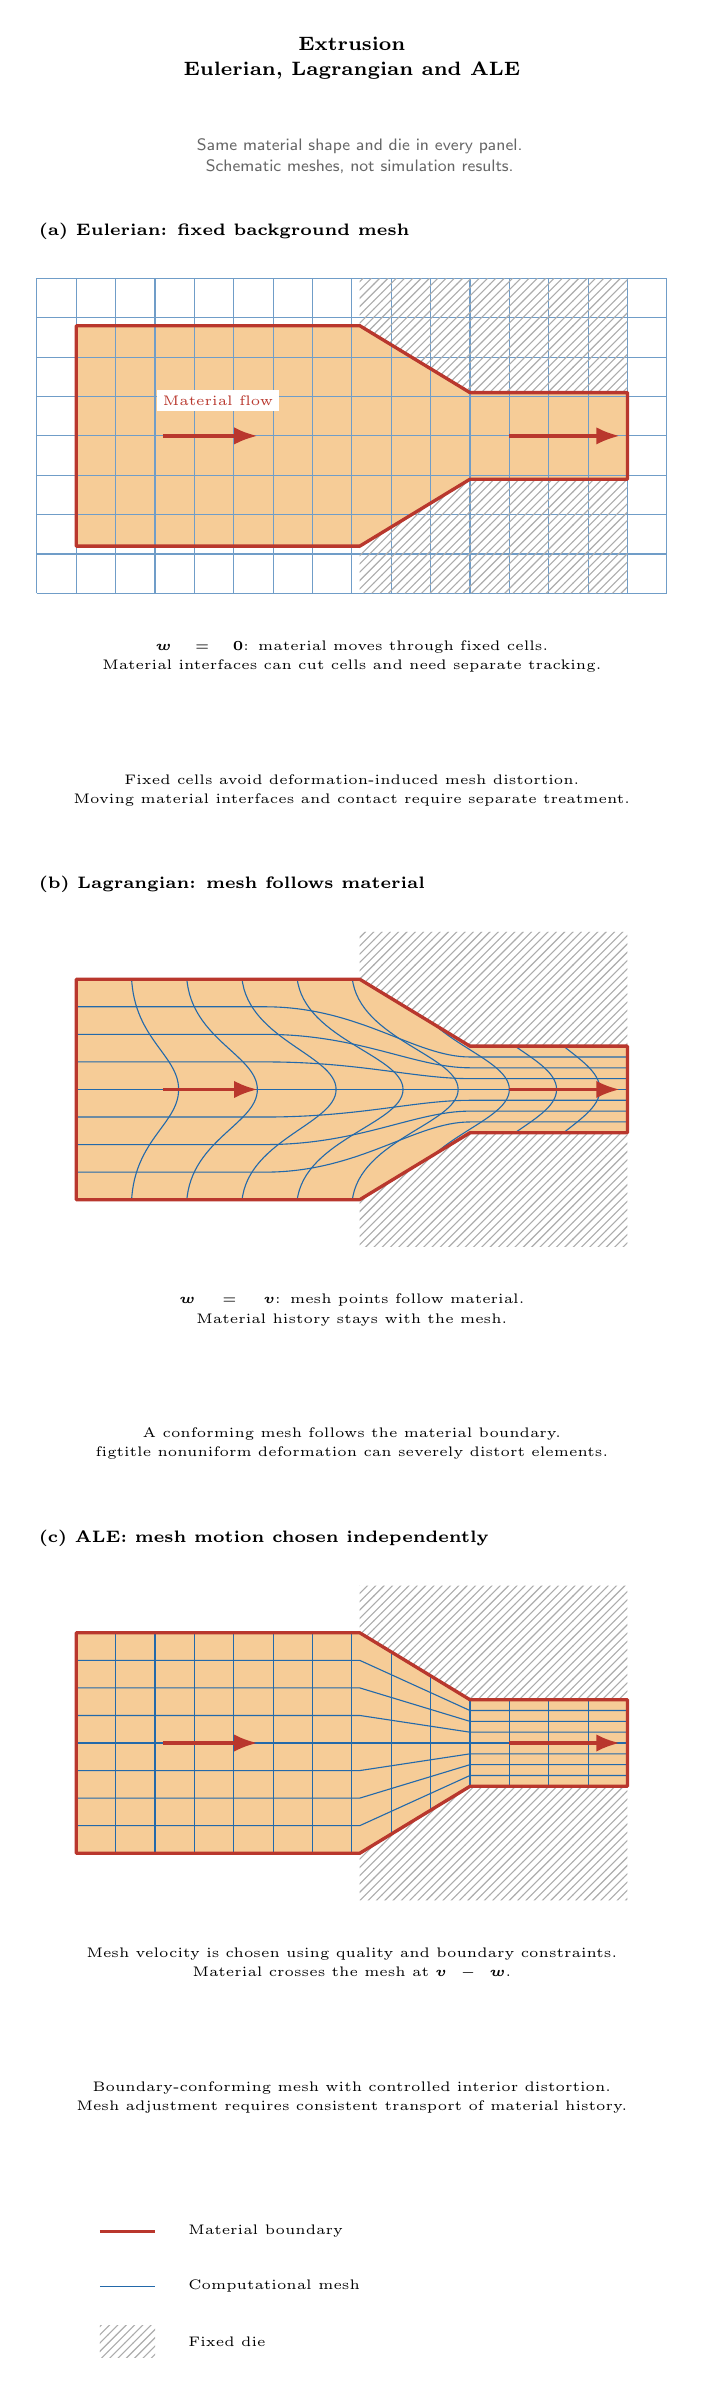
\begin{tikzpicture}[>=Latex,font=\sffamily\figtext,line join=round]
\node[font=\figtitle\bfseries,align=center] at (3.5,4.8) {Extrusion\\Eulerian, Lagrangian and ALE};
\node[text=gray!80!black,align=center] at (3.6,3.55) {Same material shape and die in every panel.\\Schematic meshes, not simulation results.};
\foreach \dy/\title in {0/{(a) Eulerian: fixed background mesh},-8.3/{(b) Lagrangian: mesh follows material},-16.6/{(c) ALE: mesh motion chosen independently}}{
\begin{scope}[shift={(0,\dy)}]
 \node[font=\figtext\bfseries,anchor=west] at (-.6,2.6) {\title};
 \fill[body] \bodypath;
\end{scope}}
% EULERIAN: fixed Cartesian cells cross the material boundary.
\begin{scope}
\draw[meshblue!65,step=.5,thin] (-.5,-2) grid (7.5,2);
\die
\draw[flow,very thick] \bodypath;
\draw[flow,->,very thick] (1.1,0)--(2.3,0);
\draw[flow,->,very thick] (5.5,0)--(6.9,0);
\node[flow,fill=white,inner sep=2pt,font=\fignote] at (1.8,.45) {Material flow};
\node[font=\fignote,align=center,text width=8cm] at (3.5,-2.8) {$\boldsymbol w=\boldsymbol0$: material moves through fixed cells.\\Material interfaces can cut cells and need separate tracking.};
\node[font=\fignote,align=center,text width=8cm] at (3.5,-4.5) {Fixed cells avoid deformation-induced mesh distortion.\\Moving material interfaces and contact require separate treatment.};
\end{scope}
% LAGRANGIAN: a stylized convected mesh with skewed elements.
\begin{scope}[shift={(0,-8.3)}]
\begin{scope}
\clip \bodypath;
\foreach \f in {-.75,-.5,-.25,0,.25,.5,.75}{
\draw[meshblue,thin] (0,{1.4*\f})--(2.4,{1.4*\f}) .. controls (3.6,{1.4*\f}) and (4.3,{.55*\f}) .. (5,{.55*\f})--(7,{.55*\f});}
\foreach \a/\c in {.7/1.3,1.4/2.3,2.1/3.3,2.8/4.15,3.5/4.85,4.2/5.5,4.9/6.1,5.6/6.65}{
\draw[meshblue,thin] (\a,-1.5) .. controls (\a,-.65) and (\c,-.45) .. (\c,0) .. controls (\c,.45) and (\a,.65) .. (\a,1.5);}
\end{scope}
\die
\draw[flow,very thick] \bodypath;
\draw[flow,->,very thick] (1.1,0)--(2.3,0);
\draw[flow,->,very thick] (5.5,0)--(6.9,0);
\node[font=\fignote,align=center,text width=8cm] at (3.5,-2.8) {$\boldsymbol w=\boldsymbol v$: mesh points follow material.\\Material history stays with the mesh.};
\node[font=\fignote,align=center,text width=8cm] at (3.5,-4.5) {A conforming mesh follows the material boundary.\\figtitle nonuniform deformation can severely distort elements.};
\end{scope}
% ALE: boundary fitted but interior mesh need not follow material.
\begin{scope}[shift={(0,-16.6)}]
\begin{scope}
\clip \bodypath;
\foreach \f in {-.75,-.5,-.25,0,.25,.5,.75}{
\draw[meshblue,thin] (0,{1.4*\f})--(3.6,{1.4*\f})--(5,{.55*\f})--(7,{.55*\f});}
\foreach \x in {.5,1,1.5,2,2.5,3,3.5,4,4.5,5,5.5,6,6.5}{\draw[meshblue,thin] (\x,-1.5)--(\x,1.5);}
\end{scope}
\die
\draw[flow,very thick] \bodypath;
\draw[flow,->,very thick] (1.1,0)--(2.3,0);
\draw[flow,->,very thick] (5.5,0)--(6.9,0);
\node[font=\fignote,align=center,text width=8cm] at (3.5,-2.8) {Mesh velocity is chosen using quality and boundary constraints.\\Material crosses the mesh at $\boldsymbol v-\boldsymbol w$.};
\node[font=\fignote,align=center,text width=8cm] at (3.5,-4.5) {Boundary-conforming mesh with controlled interior distortion.\\Mesh adjustment requires consistent transport of material history.};
\end{scope}

\draw[flow,very thick] (.3,-22.8)--(1,-22.8);
\node[anchor=west,font=\fignote] at (1.3,-22.8) {Material boundary};
\draw[meshblue,thin] (.3,-23.5)--(1,-23.5);
\node[anchor=west,font=\fignote] at (1.3,-23.5) {Computational mesh};
\fill[pattern=north east lines,pattern color=gray!65] (.3,-24.4) rectangle (1,-24);
\node[anchor=west,font=\fignote] at (1.3,-24.2) {Fixed die};
\end{tikzpicture}
\end{document}
